\documentclass[11pt,a4paper]{article}
\usepackage[margin=24mm]{geometry}
\usepackage{amsmath,amssymb,booktabs,graphicx,hyperref}
\title{Plasma-Echo-Constrained Kinetic Memory\\A Reduced-Order Falsification Framework}
\author{Devanik Debnath\\National Institute of Technology Agartala, India}
\date{10 November 2026 --- Research preprint, not peer reviewed}
\begin{document}\maketitle
\begin{abstract}
This paper studies a reduced two-pulse plasma-echo model and a synthetic delay-embedding benchmark. It distinguishes kinematic rephasing, phenomenological collisional attenuation and synthetic forecasting. It is not a self-consistent Vlasov-Poisson simulation, does not train a neural operator on kinetic data, and does not analyse laboratory or spacecraft observations. No new plasma mechanism or experimental validation is claimed.
\end{abstract}
\newpage
\section{Question and scope}
Can an echo-centred intervention distinguish a reduced state that retains recoverable phase information from one whose echo response is attenuated by a declared model? The second pulse is an intervention. The target is the later echo-mode response under pulse protocols withheld from fitting. The rephasing time is kinematic; attenuation is a model definition; forecasting is synthetic. These layers must not be conflated.
\newpage
\section{Phase mixing}
A Fourier perturbation in a freely streaming kinetic system carries the velocity phase exp(-ikvt). Velocity integration can make a low-order moment small while the distribution develops fine velocity-space structure. Cancellation is not microscopic erasure and is not by itself thermodynamic entropy production. Landau damping is self-consistent; free streaming is used only to expose echo geometry.
\newpage
\section{Established echo physics}
The plasma-wave echo was experimentally reported by Malmberg, Wharton, Gould and O'Neil in 1968. A second perturbation couples to velocity-space structure prepared by the first and generates a difference mode whose phase later rephases. Echo amplitude depends on equilibrium distribution, pulse geometry, field-particle coupling, collisions, finite amplitude and measurement bandwidth. The phenomenon is established; no priority claim is made.
\cite{Malmberg1968,Ichikawa1969,Grenier2022}
\newpage
\section{Projection memory}
For full state z(t), evolution dz/dt=R(z), and projection P onto resolved observables, with Q=I-P, Mori-Zwanzig identities express resolved dynamics through an instantaneous term, a memory integral and unresolved initial-state contributions. A finite lag window is an approximation, not the exact kernel. This release does not recover an exact kernel.
\cite{Zwanzig1961,Mori1965,Chorin2000,Burles2026}
\newpage
\section{Two-pulse derivation}
Let the first perturbation have wavenumber k1 at t=0 and the second have wavenumber k2 at t=tau. Coupling produces
\[
k_3=k_2-k_1.
\]
The velocity-dependent phase is proportional to k2*tau-k3*t. Setting it to zero gives
\[
t_e=\frac{k_2\tau}{k_2-k_1},\quad k_2>k_1>0.
\]
This is a P1 identity under the stated phase ansatz, not an amplitude theorem.
\newpage
\section{Reduced echo envelope}
Define w=1/k3 and
\[
E_3(t)=A_3\exp[-(t-t_e)^2/(2w^2)],
\quad A_3=a_1a_2(k_1/k_3)\exp[-\nu k_1^2\tau^3/3].
\]
The bilinear pulse factor is a second-order ansatz; k1/k3 is a normalization choice; the Gaussian envelope is a smooth test signal. None is a universal physical coefficient.
\newpage
\section{Collisional attenuation}
Velocity diffusion damps fine velocity-space Fourier structure at a rate proportional to the square of its velocity wavenumber. The cubic exponent is a transparent reduced proxy, not an exact Coulomb, BGK or Lenard-Bernstein echo law. No physical collision frequency is inferred from nu.
\cite{Ichikawa1969}
\newpage
\section{Synthetic memory benchmark}
A deterministic synthetic signal combines a damped oscillation, a localized Gaussian echo-like pulse and Gaussian noise. Seed 20261110 is fixed. Examples are split chronologically, 70 percent for training and 30 percent for testing. Ridge regression with the current observation is compared with a 24-sample delay window. This is not a neural network and the target is not kinetic data.
\newpage
\section{Forecast result}
Memoryless one-step RMSE is 0.0222991; 24-lag delay RMSE is 0.0160948, a 27.82 percent reduction on one synthetic holdout. This shows only that temporal context helps this constructed signal. It does not establish a physical memory kernel. A physical test needs independent kinetic trajectories and grouped holdouts.
\newpage
\section{Novelty and falsification}
A finite-memory neural-operator closure for Landau damping appeared online on 30 October 2026. This work does not claim finite-memory plasma closure is new. A next-stage study must reproduce Landau damping, run a two-pulse echo, test grid convergence, monitor invariants, compare collision operators and hold out pulse timing, wavenumber, amplitude and collisionality.
\newpage
\section{Limitations}
The reduced envelope is not a self-consistent Vlasov-Poisson solution. It omits field feedback, nonlinear trapping, physical collision operators, multidimensional geometry and instrument effects. Numerical dissipation can mimic collisional attenuation. The synthetic predictor may exploit autocorrelation rather than physical memory. No laboratory or MMS data are analysed.
\newpage
\section{Candidate table}
\begin{tabular}{lll}\toprule Candidate & Decision & Reason\\\midrule
Neural Landau closure & Reject & Direct precedent\\
Echo memory test & Select & Falsifiable intervention\\
Hermite inversion & Defer & Needs kinetic solver\\
Collision identification & Defer & Needs validated operators\\
MMS echo & Defer & No controlled pulse\\\bottomrule
\end{tabular}
\newpage
\section{Assumption table}
\begin{tabular}{lll}\toprule Assumption & Role & Boundary\\\midrule
1D kinematics & Phase cancellation & Not multidimensional\\
Free streaming & Echo geometry & No field feedback\\
Second-order pulse & Bilinear ansatz & Small-signal only\\
Gaussian envelope & Smooth signal & Not universal\\
Cubic attenuation & Diffusion proxy & Operator dependent\\\bottomrule
\end{tabular}
\newpage
\section{Verification table}
\begin{tabular}{lll}\toprule Check & Result & Meaning\\\midrule
Echo time & 6.0 & Identity check\\
Amplitude ratio & 2.0 & Model property\\
Attenuation & Monotone & Declared formula\\
Proxy sum & 1.0 & Normalization\\
Invalid k & Rejected & Input guard\\
Delay RMSE & 27.82 percent lower & Synthetic only\\\bottomrule
\end{tabular}
\newpage
\section{Literature table}
\begin{tabular}{lll}\toprule Work & Contribution & Relation\\\midrule
Malmberg 1968 & Echo experiment & Known physics\\
Ichikawa 1969 & Collisions & Operator effects\\
Grenier 2022 & Echo cascades & Nonlinear context\\
Zwanzig/Mori & Projection memory & Foundations\\
Burles 2026 & Neural closure & Adjacent prior\\\bottomrule
\end{tabular}
\newpage
\section{Falsification table}
\begin{tabular}{lll}\toprule Claim & Test & Failure\\\midrule
Echo time & Kinetic holdouts & Timing error\\
Memory gain & History shuffle & Gain vanishes\\
Collision law & Operator comparison & Resolution dependence\\
Generalization & Pulse holdouts & OOD collapse\\
Invariants & Residual checks & Excess drift\\\bottomrule
\end{tabular}
\newpage
\section{Reproducible figures}
\begin{figure}[p]\centering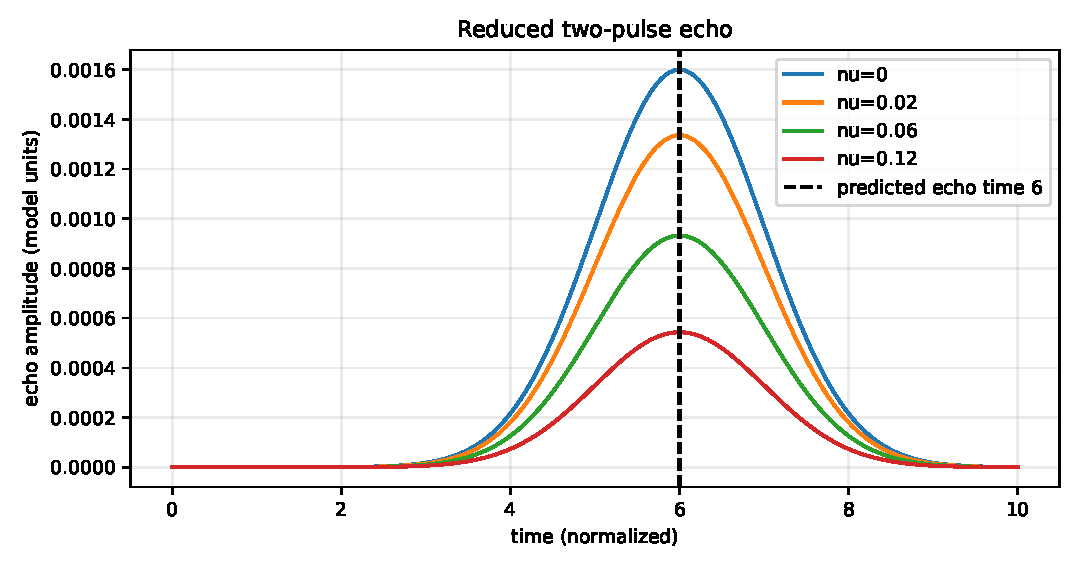
\includegraphics[width=.9\textwidth]{figures/fig1_echo_recovery.pdf}\caption{Reduced echo envelope.}\end{figure}
\newpage
\begin{figure}[p]\centering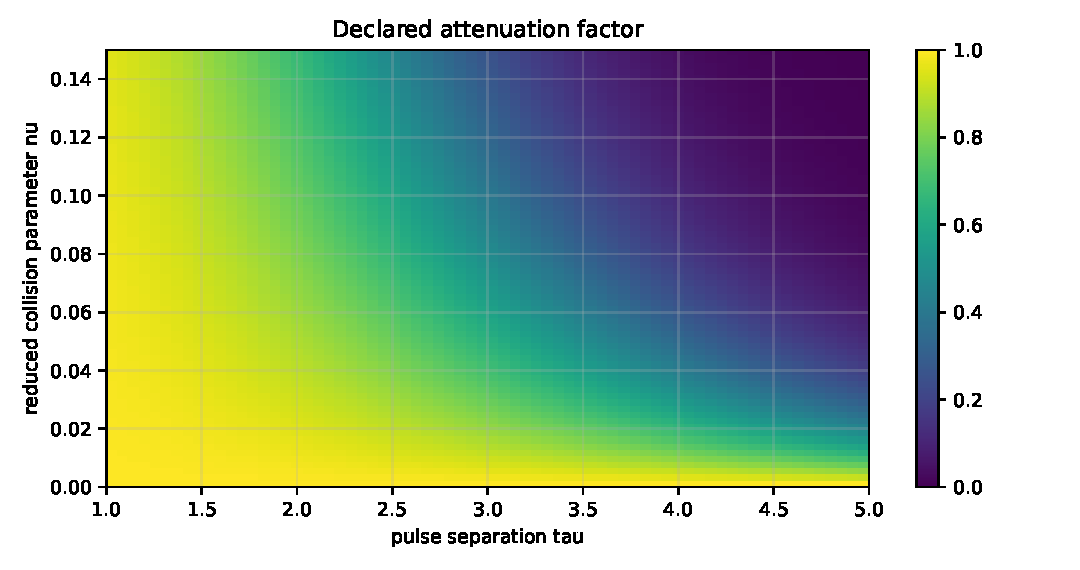
\includegraphics[width=.9\textwidth]{figures/fig2_attenuation_map.pdf}\caption{Attenuation map.}\end{figure}
\newpage
\begin{figure}[p]\centering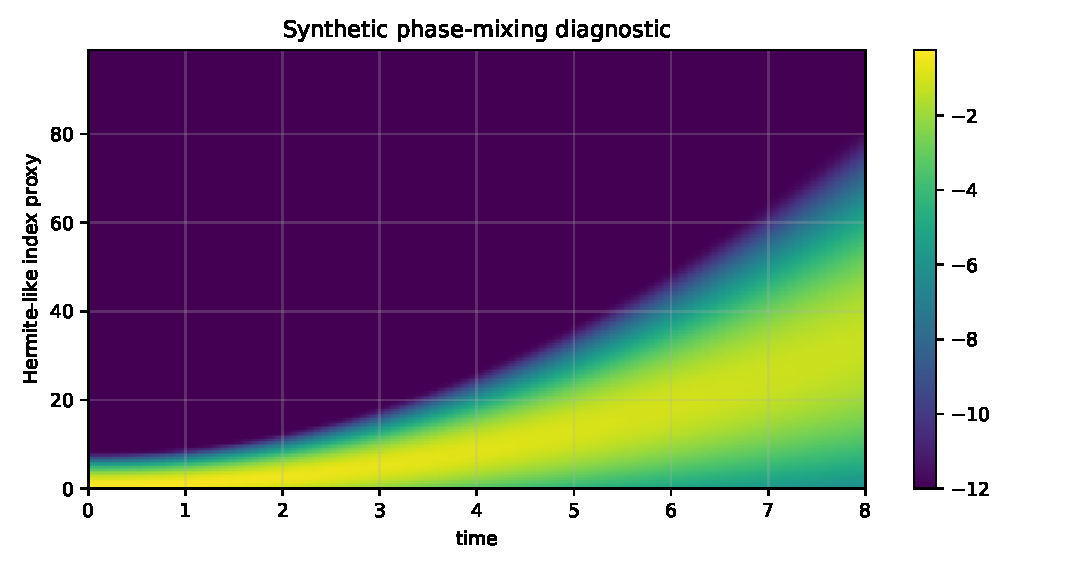
\includegraphics[width=.9\textwidth]{figures/fig3_phase_mixing_proxy.pdf}\caption{Synthetic phase-mixing proxy.}\end{figure}
\newpage
\begin{figure}[p]\centering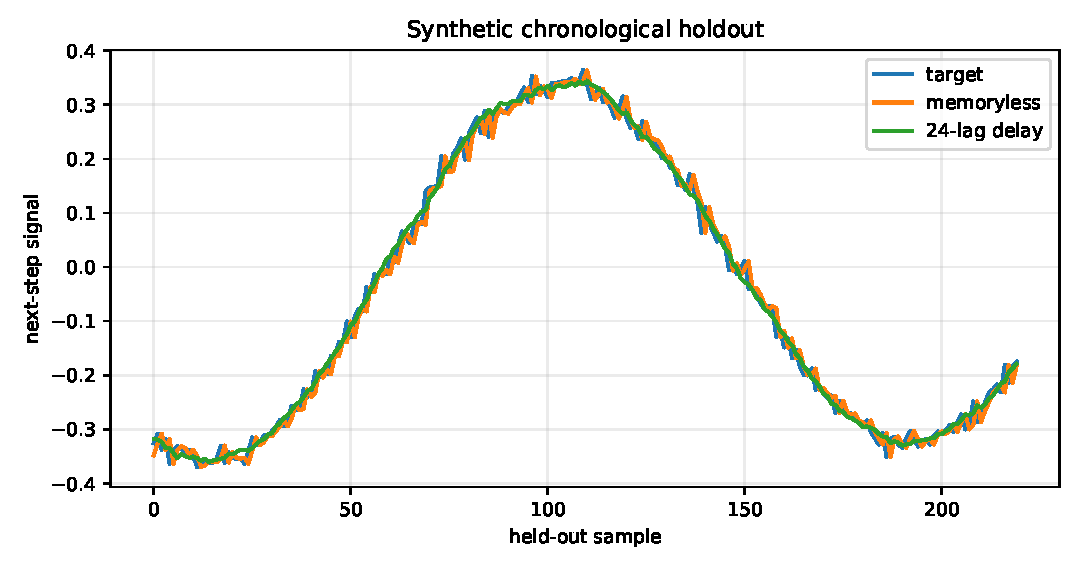
\includegraphics[width=.9\textwidth]{figures/fig4_memory_forecast.pdf}\caption{Synthetic memory forecast.}\end{figure}
\newpage
\begin{figure}[p]\centering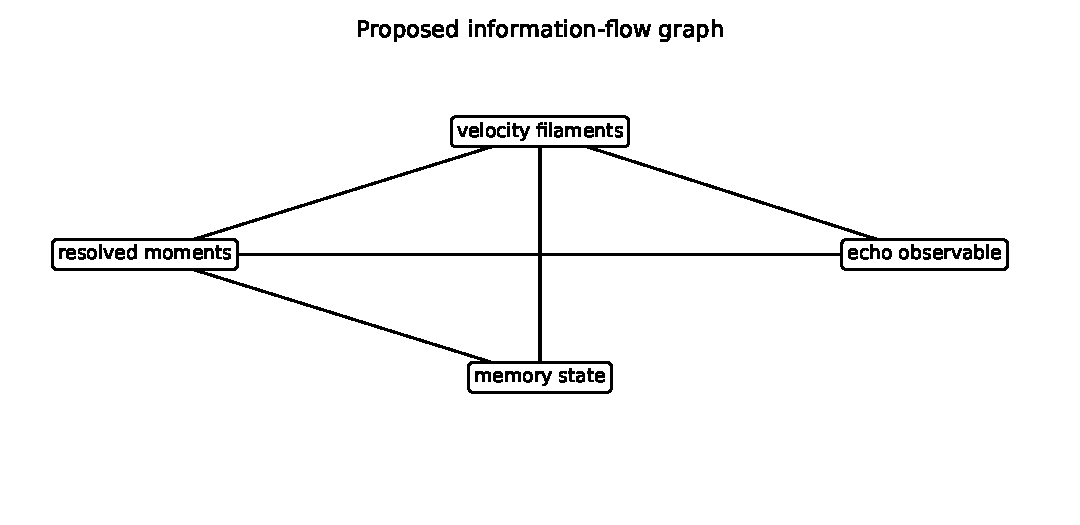
\includegraphics[width=.9\textwidth]{figures/graph1_information_flow.pdf}\caption{Information-flow graph.}\end{figure}
\newpage
\begin{figure}[p]\centering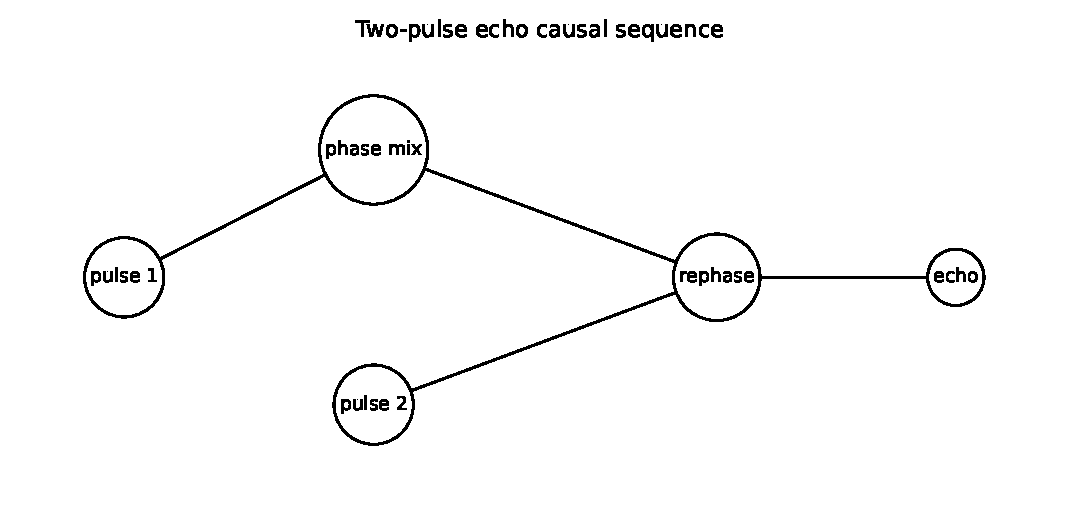
\includegraphics[width=.9\textwidth]{figures/graph2_echo_causality.pdf}\caption{Echo causal graph.}\end{figure}
\newpage
\begin{figure}[p]\centering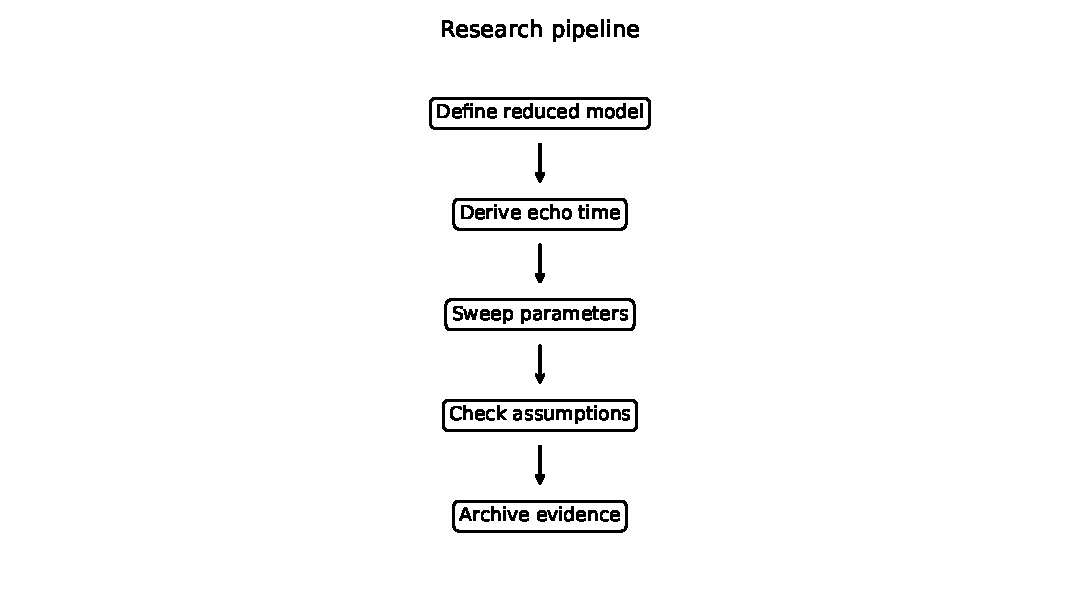
\includegraphics[width=.9\textwidth]{figures/flow1_pipeline.pdf}\caption{Research pipeline.}\end{figure}
\newpage
\begin{figure}[p]\centering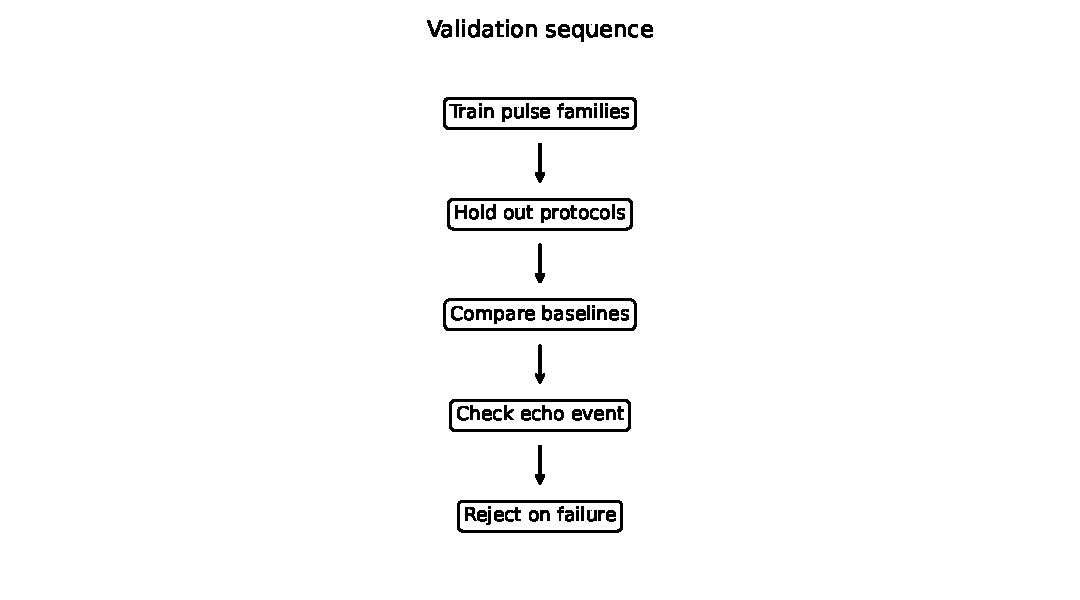
\includegraphics[width=.9\textwidth]{figures/flow2_validation.pdf}\caption{Validation flow.}\end{figure}
\newpage
\section*{Research-process disclosure}
Co-equal research-process credit is given to Devanik Debnath and Xylia, the AI-assisted research orchestration system coordinating discovery, synthesis and verification. Devanik Debnath retains responsibility for the final manuscript, scientific claims, citations and released artifacts.
\newpage
\begin{thebibliography}{9}
\bibitem[Malmberg et al. (1968)]{Malmberg1968} J. H. Malmberg et al., Phys. Rev. Lett. 20, 95 (1968), doi:10.1103/PhysRevLett.20.95.
\bibitem[Ichikawa and Suzuki (1969)]{Ichikawa1969} Y. H. Ichikawa and T. Suzuki, Prog. Theor. Phys. 41, 313 (1969), doi:10.1143/PTP.41.313.
\bibitem[Grenier et al. (2022)]{Grenier2022} E. Grenier et al., SIAM J. Math. Anal. 54, 940 (2022), doi:10.1137/21M1392553.
\bibitem[Zwanzig (1961)]{Zwanzig1961} R. Zwanzig, Phys. Rev. 124, 983 (1961), doi:10.1103/PhysRev.124.983.
\bibitem[Mori (1965)]{Mori1965} H. Mori, Prog. Theor. Phys. 33, 423 (1965), doi:10.1143/PTP.33.423.
\bibitem[Chorin et al. (2000)]{Chorin2000} A. J. Chorin et al., PNAS 97, 2968 (2000), doi:10.1073/pnas.97.7.2968.
\bibitem[Burles et al. (2026)]{Burles2026} S. Burles et al., J. Plasma Phys. (2026), doi:10.1017/S0022377826102517.
\bibitem[Vo et al. (2026)]{Vo2026} T. Vo et al., Phys. Rev. Lett. (2026), doi:10.1103/2ndf-sgy8.
\end{thebibliography}
\end{document}
